\section{Generalità sui bacini, sulla confluenza e sull'evento pluviometrico di studio}
Con bacino idrografico si intende tutta la superficie, definito un punto (sezione di chiusura), da cui proviene l'acqua di deflusso e che la attraversa. Infatti, al fine dello studio idraulico di una qualsiasi area, la conoscenza del bacino idrografico permette di conoscere la superficie di terreno da cui viene generato il runoff, che permette di quantificare il volume idrico alla sezione di chiusura, con conseguente analisi di eventuali inondazioni verso le piane alluvionali.\\
Il tratto interessato da questo studio idraulico è quello della confluenza tra il fiume Boite ed il fiume Piave, nel Comune di Perarolo (BL).\\
Vengono riportati i bacini idrogeologici dei fiumi Boite \cite{fiume_boite} e Piave \cite{fiume_piave}.
\begin{figure}[htb] \centering
    \begin{minipage}[]{7cm}
        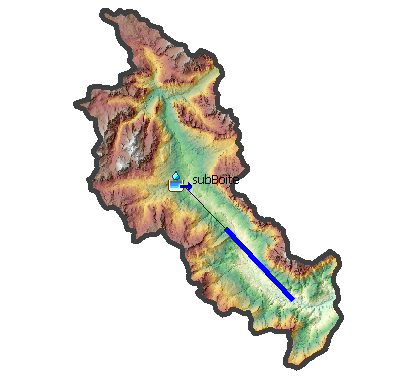
\includegraphics[scale=0.73]{immagini/bac_boite.PNG}
        \caption{Bacino idrografico del Boite.}
    \label{minipage:bacino_boite}    
    \end{minipage}
        \hspace{2cm}
    \begin{minipage}[]{7cm}
        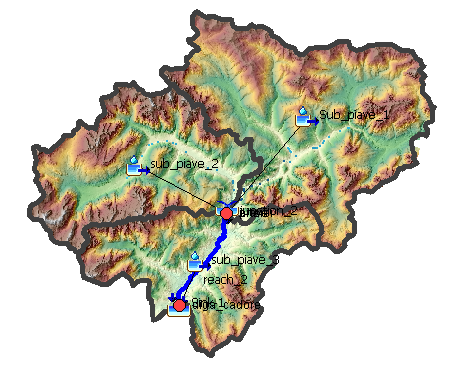
\includegraphics[scale=0.75]{immagini/bac_piave.PNG}
        \caption{Bacino idrografico del Piave.}
    \label{minipage:bacino_piave}
    \end{minipage} 
        \end{figure}

Il bacino del fiume Boite ha un'estensione di 383 \unit{km^2}, mentre il bacino del Piave ha un'estensione totale di 813 \unit{km^2}.\\
Il fiume Boite (proveniente da ovest) ed il fiume Piave (proveniente da est) generano una confluenza idraulica, come osservabile nelle seguenti immagini \eqref{minipage:confl_google_earth}\eqref{minipage:confl_dtm}.

\begin{figure}[htb] \centering
    \begin{minipage}[]{7cm}
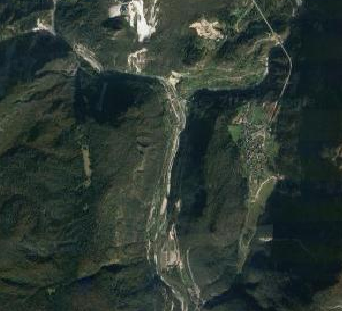
\includegraphics[scale=0.80]{immagini/confl_google_earth.PNG}
\caption{Rilievo satellitare del tratto di confluenza dei due fiumi (Google Satellite).}
\label{minipage:confl_google_earth}    
    \end{minipage}
        \hspace{2cm}
    \begin{minipage}[]{7cm}
        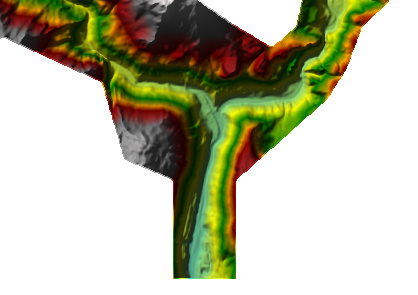
\includegraphics[scale=0.90]{immagini/confl_dtm.PNG}
        \caption{Modello digitale del terreno (DTM) della confluenza dei due fiumi.}
    \label{minipage:confl_dtm}
    \end{minipage} 
        \end{figure}
Essendo presenti delle opere idrauliche (come ponti o arginature), al fine di ottimizzare l'analisi mediante il programma HEC-RAS, è necessario riportare tali geometrie.

\begin{figure}[htb] \centering
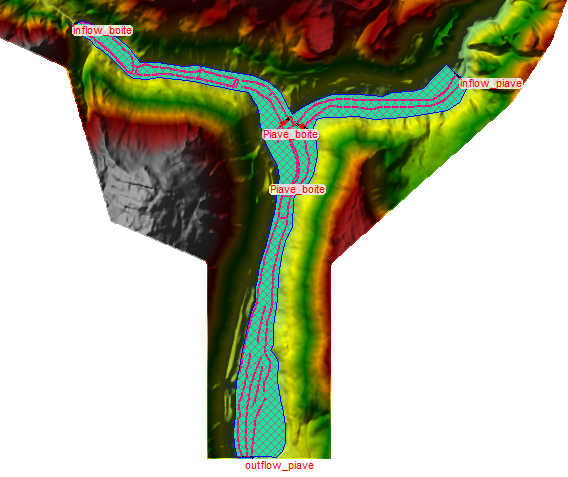
\includegraphics[scale=0.7]{immagini/confl_geom.PNG}
\caption{Geometrie presenti all'interno del dominio di calcolo del modello idraulico.}
\label{figure:confl_geom}    
\end{figure}
Nella figura \eqref{figure:confl_geom} è possibile notare:
\begin{itemize}
    \item il dominio di calcolo (l'area di colore azzurro);
    \item le breaklines delle arginature (le linee di colore rosso);
    \item i ponti del fiume Boite e Piave (di colore rosso);
    \item i volumi idrici entranti ed uscenti (inflow boite e piave ed outflow piave).
\end{itemize}
Tali concetti verranno ripresi successivamente, nel capitolo inerente al funzionamento del programma HEC-RAS.\\
Per quanto riguarda i dati da introdurre all'interno del programma, si farà riferimento all'analisi idrologica compiuta sui medesimi bacini idrografici, mediante HEC-HMS.\\
L'analisi, basata su reali dati storici, ha portato come risultati i deflussi idrologici alla sezione di chiusura dei due bacini, per un tempo di ritorno pari a 215 anni.\\
I risultati dell'analisi idrologica possono essere riassunti mediante le seguenti tabelle ed i seguenti grafici \eqref{figure:LSPP_215}\eqref{figure:boite_215}\eqref{figure:risul_boite_215}\eqref{figure:sink_piave_215}\eqref{figure:risul_piave_215}.


\begin{figure}[htb] \centering
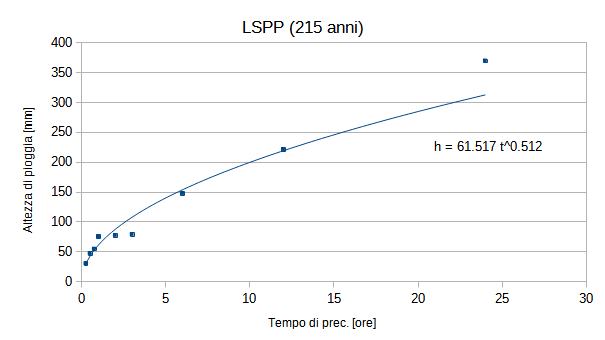
\includegraphics[scale=0.6]{immagini/LSPP_215.png}
\caption{Linea segnalatrice di probabilità pluviometrica (LSPP), per un tempo di ritorno di 215 anni.}
\label{figure:LSPP_215}    
\end{figure}

\begin{figure}[htb] \centering
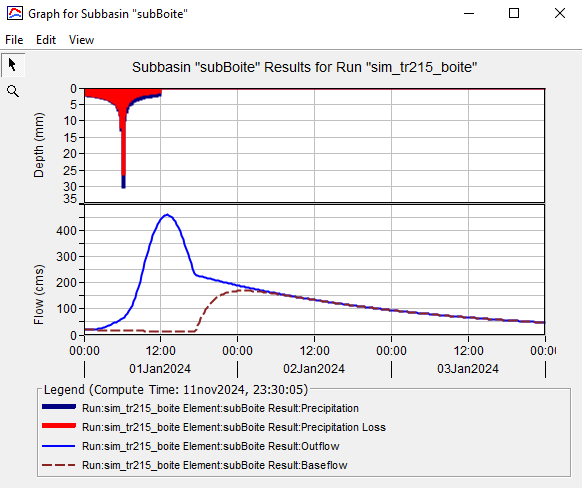
\includegraphics[scale=0.6]{immagini/boite_215.PNG}
\caption{Idrogramma alla sezione di chiusura del bacino del Boite, per il tempo di ritorno di 215 anni.}
\label{figure:boite_215}    
\end{figure}

\begin{figure}[htb] \centering
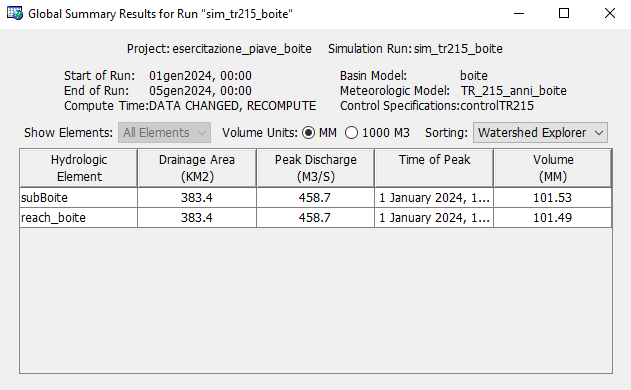
\includegraphics[scale=0.6]{immagini/risul_boite_215.PNG}
\caption{Portata di picco e volume totale transitato alla sezione di chiusura del fiume Boite, per tempo di ritorno di 215 anni.}
\label{figure:risul_boite_215}
\end{figure}

\begin{figure}[htb] \centering
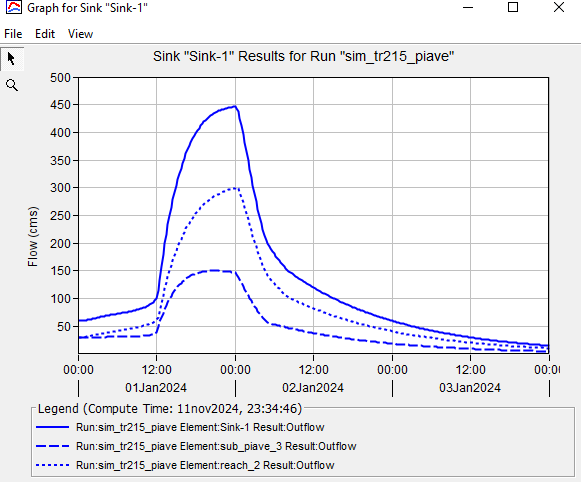
\includegraphics[scale=0.6]{immagini/sink_piave_215.PNG}
\caption{Idrogramma alla sezione di chiusura del bacino del Piave, per il tempo di ritorno di 215 anni.}
\label{figure:sink_piave_215}    
\end{figure}

\begin{figure}[htb] \centering
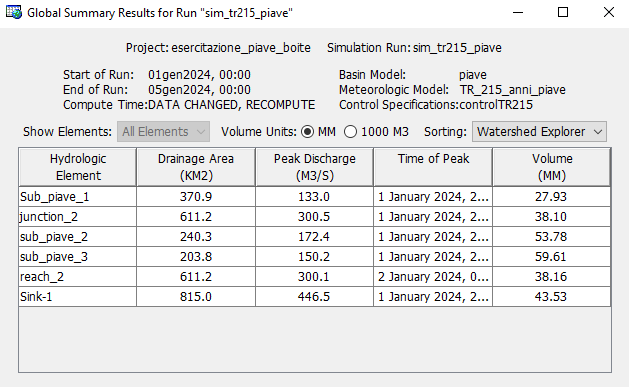
\includegraphics[scale=0.6]{immagini/risul_piave_215.PNG}
\caption{Portata di picco e volume totale transitato alla sezione di chiusura del fiume Piave, per tempo di ritorno di 215 anni.}
\label{figure:risul_piave_215}
\end{figure}

Sintetizzando, mediante l'analisi statistico-probabilistica è stata ricavata la curva LSPP per il tempo di ritorno di 215 anni; tale funzione è pari a $h=61.517 \cdot t ^{0.512}$.\\
A fronte di una precipitazione con tempo di ritorno pari a 215 anni, il bacino del Boite genera un picco di deflusso di 458.7 $m^3/s$, mentre il bacino del Piave ne genera uno complessivo di 446.5 $m^3/s$.\\
L'altro risultato importante da considerare è il volume defluito alla sezione di chiusura alla fine dell'evento pluviometrico con tempo di ritorno di 215 anni, che è pari a 101.49 mm per il bacino del Boite e 43.53 mm per il bacino del Piave.